\chapter{User-Space Runtime and Detection Implementation}
\label{ch:user-space-implementation}

Chapter~4 described how the eBPF programs construct and submit binary event
records through the perf buffer. This chapter starts at the corresponding
user-space boundary. It explains how the Go runtime turns the selected monitoring configuration into
a managed user-space pipeline, from program preparation and record
interpretation to policy-driven analysis, detector evaluation, and the delivery
of monitoring and diagnostic results.

\section{Command-Line Configuration and Runtime Bootstrap}

The user-space workflow begins at the command-line interface, implemented with
  the Cobra library for Go \cite{spf13_cobra}. Its purpose is to translate
  operator input into one configuration object shared by the subsequent runtime
  components. Cobra is responsible only for command definition, argument parsing and invocation of
  the application entry point; it does not load policies, evaluate detectors or
  attach eBPF programs.

  The configuration is initialised with defaults suitable for the target
  environment. These include the host BTF path, JSON event and alert output,
  console-formatted operational logs and an informational log level. CLI flags
  then update the corresponding fields for event selection, kernel-side
  filtering, policy and detector paths, output behaviour, logging and eBPF input
  selection. Keeping these values in one typed structure avoids passing an
  independent collection of command-line values through the runtime.

  Before any kernel-facing resource is acquired, the configuration passes
  through normalisation and static validation. Normalisation derives internal
  settings from the operator's intent. Supplying one or more detector paths
  automatically enables detector processing, while selecting
  \texttt{alerts-only} also enables alert generation. Validation then rejects
  unsupported event-output, alert-output and logging formats. This ordering
  prevents malformed configuration from reaching eBPF loading or attachment.

  The command also separates informational execution from active monitoring.
  The \texttt{list-events} option obtains the public event names from the probe
  registry and exits without resolving BTF, opening the eBPF object or attaching
  programs. A normal monitoring invocation instead resolves the eBPF object,
  constructs the application runner and transfers ownership of the validated
  configuration to it.

  Listing~\ref{lst:cobra-runtime-handoff} summarises this control flow.

  \begin{lstlisting}[
      language=Go,
      caption={Validated handoff from the Cobra command to the runtime
      (abridged).},
      label={lst:cobra-runtime-handoff}
  ]
  if err := ValidateConfig(&cliCfg); err != nil {
      return err
  }
  if cliCfg.ListEvents {
      printSupportedEvents(cmd.OutOrStdout())
      return nil
  }
  if err := initialize.BPFObject(&cliCfg); err != nil {
      return err
  }
  runner, err := NewProjectRunner(cliCfg)
  if err != nil {
      return err
  }
  return runner.Run(ctx)
  \end{lstlisting}

  This staged bootstrap follows a fail-fast design. Errors in static
  configuration, external definitions or runtime construction are reported
  before active monitoring begins whenever possible. Record-local failures that
  occur after startup belong instead to the event-processing lifecycle described
  later in this chapter.

\section{Loader, Probe Registry and Attachment Lifecycle}
\label{sec:implementation-loader-registry}

After the command-line layer has produced a validated configuration, the
  bootstrap process resolves the inputs required by the eBPF runtime. An external
  object specified through \texttt{PROJECT\_BPF\_OBJECT} has precedence over the
  command-line path; otherwise, the object embedded in the executable is used.
  The BTF path follows the corresponding environment, command-line and default
  host-path order. Embedding simplifies distribution, but loading still requires
  compatible host BTF, kernel facilities and privileges.

  Policy and detector definitions are prepared before the eBPF module is opened.
  A policy with an explicit event scope can narrow the CLI selection, while an
  open-ended rule retains the broader scope. If the exact policy scope and CLI
  selection do not overlap, startup fails instead of interpreting an empty set as
  a request for all events. Detector selection does not independently enable additional kernel
  events: its inputs must already belong to the effective monitoring scope.

  The probe registry converts the selected logical events into the eBPF programs
  required for collection. A selected event may also require internal support probes that
  collect intermediate information without producing a public event.

  Listing~\ref{lst:probe-plan} shows how the registry includes both directly
  selected programs and their internal dependencies.

  \begin{lstlisting}[
      language=Go,
      caption={Selection of producer and support probes (abridged).},
      label={lst:probe-plan}
  ]
  for _, probe := range supportedProbes {
      if probeActivation[probe.eventName] {
          selectedProbes = append(selectedProbes, probe)
          continue
      }
      for _, event := range probe.impliedBy {
          if probeActivation[event] {
              selectedProbes = append(selectedProbes, probe)
              break
          }
      }
  }
  \end{lstlisting}

  Registry tests verify that public events select the expected producers 
  and support probes. The actual availability of a kernel hook, however, 
  can only be established when the program is loaded and attached on the target system.

  Before the eBPF object is loaded, autoload is disabled for registered programs
  that are not part of the probe plan. Libbpf therefore loads and verifies only
  the selected producers and their dependencies. This optimisation applies to
  programs represented in the registry.

  After loading, the runtime configures the required maps, creates the perf-event
  reader and attaches each selected program to its kernel hook. Monitoring
  continues until the runtime context is cancelled, normally by
  \texttt{SIGINT} or \texttt{SIGTERM}.

\section{User-Space Decoder and Event Registry}
\label{sec:implementation-decoder-registry}

Chapter~4 described how the eBPF programs construct and submit binary event
  records. In user space, the perf reader receives those records as byte slices.
  The decoder must therefore validate their structure and convert them into the
  typed representation consumed by the rest of the Go runtime.

  Figure~\ref{fig:userspace-decoder-record-layout} shows the record regions
  processed by the decoder. The first 136 bytes contain the common event context.
  Byte 136 declares the number of arguments, while the remaining bytes contain
  the variable-length stream of indexed argument records.

  \begin{figure}[H]
      \centering
      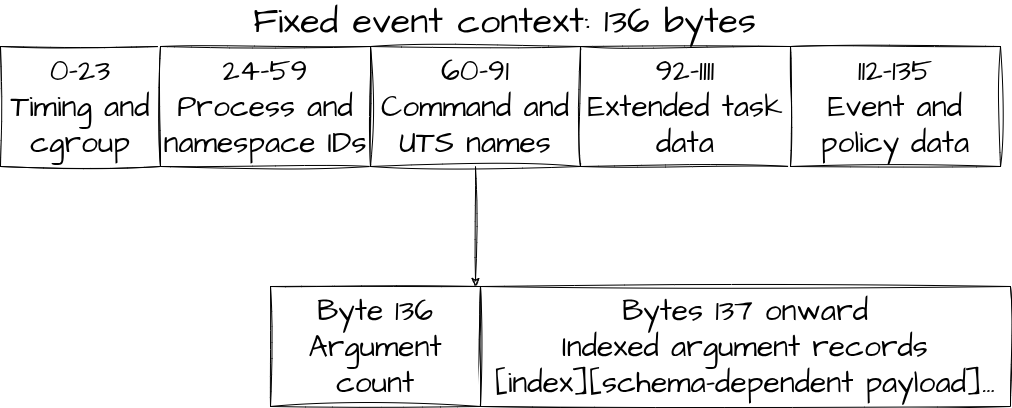
\includegraphics[
          width=0.90\textwidth,
          height=0.65\textheight,
          keepaspectratio
      ]{figures/chapter5/userspace-decoder-record-layout.drawio.png}
      \caption[Binary record layout consumed by the user-space decoder]
      {Binary record layout consumed by the user-space decoder.}
      \label{fig:userspace-decoder-record-layout}
  \end{figure}

  Before reading any field, the decoder verifies that the complete fixed context
  is available. It then interprets the header through explicit little-endian
  offsets. Fields are not obtained by copying the byte region directly into a Go
  structure, because compiler-defined padding and alignment could make the Go
  layout differ from the representation produced in C.

  The decoded context includes timing and process identity, namespace
  identifiers, command and UTS names, the numeric event identifier, the
  associated syscall and other collection metadata. The event identifier is then
  used to query the user-space event registry.

  The registry associates each public event identifier with a logical name and
  an ordered argument schema. Every schema entry defines the name and expected
  type of one event-specific argument. This registry is necessary because the
  wire representation does not include a type tag for each value.

  Each argument record begins with a one-byte index followed by its payload. The
  index selects an entry from the event schema, and the declared type determines
  how the following bytes must be decoded. Scalar values use fixed widths,
  whereas strings, byte sequences and arrays carry bounded length information.
  Socket addresses and credential snapshots use dedicated structured decoders.

  \begin{lstlisting}[
      language=Go,
      basicstyle=\ttfamily\footnotesize,
      caption={Schema-directed decoding of indexed event arguments.},
      label={lst:indexed-argument-decoding}
  ]
  spec, ok := events.GetSpec(eventID)
  if !ok {
      return nil, fmt.Errorf("unknown event id=%d", eventID)
  }

  for seen := 0; seen < argnum && offset < len(rawArgs); seen++ {
      index := int(rawArgs[offset])
      offset++

      if index >= len(spec.Args) {
          return nil, fmt.Errorf("argument index out of range")
      }

      argSpec := spec.Args[index]
      value, consumed, err :=
          decodeArgRecord(rawArgs[offset:], argSpec.DecodeAs)
      if err != nil {
          return nil, err
      }

      offset += consumed
      decoded[index] = Argument{
          Name:  argSpec.Name,
          Type:  argSpec.DecodeAs,
          Value: value,
      }
  }
  \end{lstlisting}

  A successfully decoded record becomes a
  \texttt{bufferdecoder.Event}. This structure contains the common context,
  public logical-event name and typed argument slice. It is the normalised event
  representation passed to policy matching, detector evaluation and event
  output; the presentation layer does not perform a separate event
  normalisation step.

\section{User-Space Event Selection and Admission}
\label{sec:userspace-event-selection}

After decoding, the runtime applies three short-circuit admission gates. The
first checks whether the decoded logical name belongs to the selected event
set. The second applies an optional exact command-name filter. The third asks
the policy manager whether the event is selected by the active policy set. A
policy evaluates its common scope and then its rules; matching suppress rules
override monitor or detect rules. With no configured policies, this final gate
is permissive.

Listing~\ref{lst:event-admission} shows the admission order and the resulting
fan-out. Diagnostics and optional socket enrichment are omitted because they
do not change the host-event admission contract.

\begin{lstlisting}[
    language=Go,
    caption={Decoded-event admission and consumer fan-out (abridged).},
    label={lst:event-admission}
]
event, err := bufferdecoder.DecodeEvent(raw)
if err != nil {
    return
}
if !p.eventEnabled(event.EventName) {
    return
}
if !p.commEnabled(event.Context.CommString()) {
    return
}
if !p.policyEnabled(event) {
    return
}
if !p.cfg.Alerts.Only {
    if err := p.printer.Print(event); err != nil {
        p.logger.Error("print event", zap.Error(err))
    }
}
p.processDetectors(ctx, event)
\end{lstlisting}

An admission failure prevents both normalised-event presentation and detector
evaluation.

The policy manager is intentionally not a detector. The current policy modes record monitor, detect or
suppress intent, but monitor and detect matches share the same admission path.
Suppression is the only mode that removes a matching event from subsequent
consumers.

The active loop distinguishes valid rejections from failures. At debug level,
only the first few filter drops are logged in order to avoid unbounded
diagnostic output. Decode errors, detector errors and rendering errors are
logged separately, while the loop remains active. This behaviour is established
by code inspection and component tests; a direct end-to-end unit test for the
complete admission order is still absent.

\section{Policy and Detector Engine}
\label{sec:implementation-policy-detector}

\subsection{YAML Policy and Detector Definitions}
  \label{subsec:implementation-yaml-definitions}

Policies and detectors are supplied as separate YAML documents. Both
  documents are validated and converted into internal Go models before event
  processing begins.

  Listing~\ref{lst:policy-yaml-schema} shows the principal policy fields.

  \begin{lstlisting}[
      style=thesis-yaml,
      caption={Representative YAML policy structure.},
      label={lst:policy-yaml-schema}
  ]
  name: privileged-file-monitoring
  mode: detect
  intent: threat_hunting

  scope:
    uids: [0]

  rules:
    - name: sensitive-files
      events:
        include: [security_file_open]
      filters: ["args.pathname=/etc/*"]

  detectors:
    include:
      severities: [high, critical]
      techniques: [T1548]
      stateful: true
    exclude:
      tags: [experimental]
  \end{lstlisting}

  The policy \texttt{name}, \texttt{mode} and \texttt{intent} describe its
  identity and operational purpose. Mode and intent default to
  \texttt{monitor} and \texttt{threat\_hunting}. The optional \texttt{scope}
  applies command or UID constraints to every rule.

  Rules are alternatives, while the fields within one rule are combined as
  constraints. Event exclusions take precedence over inclusions, and an empty
  include list initially admits every event. Argument filters use the
  \texttt{args.<name>} form and are evaluated after decoding because they depend
  on typed event arguments.

  The optional \texttt{detectors} block selects definitions by identifier,
  severity, tags, statefulness or MITRE ATT\&CK metadata. Values within one
  criterion are alternatives, whereas different criteria must all match.
  The exclusion block removes matching definitions from the resulting catalogue.
  Suppression policies cannot select detectors.

  A detector document defines its input events, matching logic, alert metadata
  and optional ATT\&CK classification. Listing~\ref{lst:detector-yaml-schema}
  shows a shortened collective detector.

  \begin{lstlisting}[
      style=thesis-yaml,
      caption={Representative YAML definition of a collective detector.},
      label={lst:detector-yaml-schema}
  ]
  id: privilege-exec-chain
  name: Privilege change followed by execution
  requires:
    - {event: security_task_fix_setuid,
       reason: observes a UID transition}
    - {event: sched_process_exec,
       reason: confirms executable replacement}
  consumes: [security_task_fix_setuid, sched_process_exec]

  stateful: true
  window: 5s
  group_by: [process_tree]
  steps:
    - event: security_task_fix_setuid
      conditions:
        - {field: args.new_euid, operator: eq, value: "0"}
    - event: sched_process_exec
      conditions:
        - {field: uid, operator: eq, value: "0"}

  output:
    title: Privilege change followed by process execution
    severity: high
  threat:
    tactics: [{id: TA0004, name: Privilege Escalation}]
    techniques: [{id: T1548,
                  name: Abuse Elevation Control Mechanism}]
  tags: [process, collective, privilege-escalation]
  \end{lstlisting}

  The stable \texttt{id} is used for detector selection and alert attribution.
  The \texttt{requires} entries document why events are needed, while
  \texttt{consumes} defines the set used for event dispatch. If
  \texttt{consumes} is omitted, it is derived from requirements and sequence
  steps.

  Stateless detectors place predicates in a top-level \texttt{conditions} list.
  Collective detectors use ordered \texttt{steps}, a bounded \texttt{window} and
  one or more \texttt{group\_by} strategies. The latter can correlate events by
  process, immediate process relationship, file resource, local cgroup or a
  combination of these dimensions. The corresponding correlation strategies 
  and state limits are described in Subsection~\ref{subsec:implementation-correlation-deduplication}.

  The \texttt{output} block defines the generated alert, while \texttt{threat}
  carries optional MITRE ATT\&CK classification. Conditions, event names,
  severity values, ATT\&CK identifiers and correlation plans are validated and
  compiled during startup.

  Files may be supplied directly or through directories scanned
  non-recursively in lexical order.

\subsection{Point and Collective Evaluation Paths}
  \label{subsec:implementation-point-collective}

  The conceptual distinction between point and collective detectors was
  introduced in Subsection~\ref{subsec:point-collective-detectors}. In the
  implementation, both forms satisfy the same \texttt{Detector} interface and
  enter through the same event-indexed dispatcher. The distinction is made
  inside the YAML-backed detector when an admitted event is evaluated.

  Listing~\ref{lst:detector-evaluation-path} shows the branch that separates
  immediate point evaluation from stateful sequence processing.

  \begin{lstlisting}[
      language=Go,
      caption={Selection of the point or collective evaluation path.},
      label={lst:detector-evaluation-path}
  ]
  if !d.consumes(event.EventName) {
      return nil, nil
  }

  if d.isStatefulSequence() {
      return d.onStatefulEvent(event)
  }

  matches, err := d.matches(event)
  if err != nil || !matches {
      return nil, err
  }

  return []detectors.Alert{d.newAlert(event)}, nil

  func (d *Detector) isStatefulSequence() bool {
      return d.def.Stateful && len(d.steps) > 1
  }
  \end{lstlisting}

  The first check protects the detector boundary even though the dispatcher has
  already narrowed the candidate set. The second check performs the actual
  classification: a detector uses the collective path only when it is marked as
  stateful and contains more than one compiled step. Setting
  \texttt{stateful: true} without a multi-step sequence is therefore not
  sufficient to create a collective detector.

  Collective definitions are delegated to \texttt{onStatefulEvent}. This path
  derives the configured correlation keys, looks for an existing partial
  sequence and tests the event against its next expected step. It may advance an
  existing sequence, complete it and emit its ordered evidence, or create a new
  partial sequence when the first step matches.

\subsection{Compiled Correlation State and Alert Deduplication}
  \label{subsec:implementation-correlation-deduplication}

  Chapter~3 introduced the local identities used to relate events. In the
  implementation, the YAML \texttt{group\_by} values are compiled into a
  correlation plan when the detector is constructed. Event-time processing
  therefore executes preselected key extractors rather than repeatedly parsing
  strategy names.

  The supported components produce the following internal values:

  \begin{itemize}
      \item \texttt{process} combines the host PID and task start time;
      \item \texttt{process\_tree} can additionally produce the immediate
      parent's host PID and start time when looking up an existing sequence;
      \item \texttt{resource} combines the device and inode arguments;
      \item \texttt{cgroup} uses the local kernel cgroup identifier.
  \end{itemize}

  When several components are configured, their values are joined into one
  composite key. Every component must be available: missing process, resource or
  cgroup data prevents the event from advancing the sequence instead of causing
  a fallback to a weaker identity.

  Plan construction also validates the selected strategies. Unknown or duplicate
  components are rejected, and resource correlation is accepted only when every
  sequence step exposes both \texttt{dev} and \texttt{inode}. The unsupported
  \texttt{user\_session} strategy is rejected because the event model does not
  provide a stable session identifier; UID is deliberately not used as an
  approximation.

  Each collective detector owns a map from correlation keys to partial sequence
  state. A state entry stores the next expected step, the time at which the
  sequence began and the ordered evidence already matched. Listing
  \ref{lst:collective-transition} shows how an incoming event advances one of
  these entries.

  \begin{lstlisting}[
      language=Go,
      caption={Advancement of a partial collective sequence (abridged).},
      label={lst:collective-transition}
  ]
  for _, key := range lookupKeys {
      state, ok := d.state[key]
      if !ok {
          continue
      }
      if now.Sub(state.firstSeen) > window {
          delete(d.state, key)
          continue
      }

      matches, err :=
          stepMatches(event, d.steps[state.nextStep])
      if err != nil {
          return nil, err
      }
      if !matches {
          continue
      }

      state.events = append(state.events, event)
      state.nextStep++

      if state.nextStep >= len(d.steps) {
          delete(d.state, key)
          return []detectors.Alert{
              d.newAlertFromEvents(state.events),
          }, nil
      }

      d.state[key] = state
      return nil, nil
  }
  \end{lstlisting}

  For process-tree correlation, the lookup keys may contain both the current
  process and its immediate parent. This allows an event generated by a child to
  advance state previously created for its parent without constructing a
  persistent process graph. If no existing state advances, an event matching the
  first step creates a new entry under its initial correlation key. Only one
  partial sequence is retained for each key.

  Table~\ref{tab:correlation-bounds} collects the limits applied to this state.
  These values are implementation safeguards and are not performance results.

  \begin{table}[H]
      \centering
      \small
      \renewcommand{\arraystretch}{1.15}
      \begin{tabularx}{\textwidth}{
          @{}p{0.27\textwidth}p{0.21\textwidth}X@{}}
          \toprule
          \textbf{Mechanism} & \textbf{Value} & \textbf{Runtime effect} \\
          \midrule

          Stateful window &
          2-second default; 5-second maximum &
          Bounds the lifetime of incomplete evidence. Longer definitions are
          rejected during validation. \\

          Periodic pruning &
          \texttt{min(window/2, 1 second)} &
          Avoids scanning the complete state map for every event. The directly
          addressed entry is still checked immediately. \\

          Sequence capacity &
          4,096 keys per detector &
          Inserting a new key at capacity evicts the oldest incomplete sequence. \\

          Alert deduplication &
          5-second suppression window &
          Prevents repeated equivalent alerts from being emitted during the
          configured interval. Entries older than 10 seconds are removed when
          later alert batches are processed. \\

          \bottomrule
      \end{tabularx}
      \caption{Runtime bounds for collective state and alert deduplication.}
      \label{tab:correlation-bounds}
  \end{table}

  Expired state is removed when its key is addressed and through periodic pruning
  triggered by relevant event processing. Although the detector interface exposes
  a \texttt{Flush} operation, the production runtime does not schedule it with an
  independent timer. Completely idle stale entries may therefore remain allocated
  until later relevant traffic or capacity pressure causes cleanup.

  Alert deduplication runs after detector evaluation and is separate from
  sequence correlation. Its key contains detector identity, title, severity and
  the fields of the first evidence event, while timestamps and thread identifiers
  are excluded. A repeated key inside the suppression window is not emitted.

  This mechanism reduces repeated alert output, but it does not represent the
  complete collective sequence or a durable causal identity. The deduplication
  map also has no independent capacity limit, which remains an implementation
  constraint to consider during evaluation.

\section{Output and Structured Logging}
\label{sec:implementation-output-logging}

The output package is a presentation boundary, not another normalisation stage.
It adapts the decoded event into JSON or compact text and adapts a detector
alert into a user-facing record containing detector identity, severity, ordered
evidence and optional threat metadata. JSON preserves typed values and may add
readable labels, whereas compact text is intended for interactive inspection.
The event model used by output is derived from the same decoded representation
used by policies and detectors.

Normalised event output and alert output both use standard output. They are
configured independently and can therefore use different formats in one run;
the resulting stream is not guaranteed to be one homogeneous machine-readable
schema. The \texttt{alerts-only} option suppresses normalised event output but
leaves detector evaluation and alert rendering active. Point alerts expose one
source event, while collective alerts retain their ordered evidence in JSON and
render a bounded sequence in compact text.

Operational diagnostics follow a separate path. The Zap logger writes to
standard error in console or JSON form, with debug, info, warn and error
levels. It receives runtime lifecycle messages, selected libbpf diagnostics,
perf-buffer loss notifications, decoding failures, detector failures and
presentation failures \cite{uber_zap}. Zap does not serialise monitored events
or alerts. This prevents infrastructure errors from being mistaken for security
observations and allows diagnostics to change without changing the data model
seen by event and alert consumers.

Table~\ref{tab:output-boundaries} summarises the operating channels and error
boundaries. Fatal configuration and startup failures are returned to the command
entry point, while most record-local failures are logged and the loop continues.
Logger synchronisation errors are currently discarded, so the design does not
claim durable delivery of every diagnostic message.

\begin{table}[H]
    \centering
    \small
    \renewcommand{\arraystretch}{1.16}
    \begin{tabularx}{\textwidth}{@{}p{0.22\textwidth}p{0.22\textwidth}p{0.16\textwidth}X@{}}
        \toprule
        \textbf{Class} & \textbf{Source model} & \textbf{Channel} &
        \textbf{Failure behaviour} \\
        \midrule
        Normalised event & \texttt{bufferdecoder.Event} through a printer &
        stdout & A write failure is diagnosed; subsequent events continue. \\
        Detector alert & Detector alert with one event or ordered evidence &
        stdout & A rendering failure is diagnosed; it does not change detector
        state. \\
        Operational diagnostic & Runtime, decoder, detector, output or libbpf
        condition & stderr through Zap & Record-local conditions are logged
        without becoming security events. \\
        Fatal bootstrap or lifecycle error & Command, definition loading or
        runtime setup return value & stderr through the command path & Startup
        or shutdown reports an error; cleanup errors are joined where available.
        \\
        \bottomrule
    \end{tabularx}
    \caption{User-space output and diagnostic boundaries.}
    \label{tab:output-boundaries}
\end{table}

\section{User-Space Implementation Summary}
\label{sec:user-space-implementation-summary}

The user-space implementation turns a selected perf-buffer record into a
typed event, applies explicit admission gates, and then routes admitted
evidence to presentation and deterministic detection. Policies control scope
and suppression, while detectors evaluate point conditions or bounded local
sequences and attach ATT\&CK classification metadata to their alerts. The
runtime keeps kernel-facing resource ownership, record interpretation,
analytical state and presentation responsibilities separate.

The implementation also defines clear boundaries for the following evaluation.
The registry and decoder tests establish important structural invariants, but
attachment behaviour, output under workload, alert quality, loss and resource
consumption require target-environment evidence. Chapter~6 evaluates these
behaviours on the stated Rocky Linux environment.
